%=== CHAPTER SIX (6) ===
%=== Conclusion and Recommendations ===

\chapter{Conclusion and Recommendations}
\begin{spacing}{1.5}
\setlength{\parskip}{0.3in}

\section{Unconcluded Doc}

Advanced-driver-assistance system (ADAS) plays an important role in newly designed smart cars to reduce road fatalities by minimizing human error. ADAS systems use in-vehicle cameras to capture the real-time images of roads~\cite{ziebinski2016survey}. Captured images will be handled by detection module, which recognizes lane outlines and road markings, and then respond to drivers accordingly. Current detection algorithms in deep learning are led by CNN-like network, e.g. RCNN~\cite{girshick2014rich} and its variance f-RCNN~\cite{girshick2015fast}. We also start from this structure.

Here is a sample of table in \autoref{tabelsample}

\begin{table}[ht]
\centering
\caption{A table without vertical lines.}
\label{tabelsample}
\begin{tabular}[t]{lcc}
\hline
&Treatment A&Treatment B\\
\hline
John Smith&1&2\\
Jane Doe&--&3\\
Mary Johnson&4&5\\
\hline
\end{tabular}
\end{table}%

There are several common issues in aforementioned detection process. 

First is extreme weather and bad illumination conditions. In raining days, images captured by ADAS’s camera may be blurry or be stained by raindrops, and the water on the road may lead to reflection of lights. In dusk, sun is dim, and the scene is dark-some. The road markings and lane outlines cannot be distinguished from background easily. With such distortions, the detection algorithm cannot see roads accurately. Consequently, taking measures to denoising is of vital importance. 

Second is curved road. Traditional lane detection algorithms usually work well on straight lane but will meet performance drop once the road turns quickly. VPGNet~\cite{lee2017vpgnet} used vanishing point information to solve this problem. Vanishing point is the visual intersection of two parallel lines~\cite{barnard1983interpreting}, here it is treated as the unseen end of the road.  Inspired by the intuition that human eyes utilize the vanishing point to predict the road trending, VPGNet tried to feed this information into neural network by multi-task method. They use multi-task because features employed by VP task, like road curving angle and trending, may also be useful in the detection of lanes and road markings. Based on this, we can expect that with VP information given, the Neural Network can converge better on the other two tasks (lane detection, road marking detection). But VPGNet’s VP feeding scheme is simple, not as efficient as expected. We proposed a new scheme to train with VP information. I also try to refer to this image in \autoref{fig:boundingboxexample}.


\begin{figure}[ht]
\centering
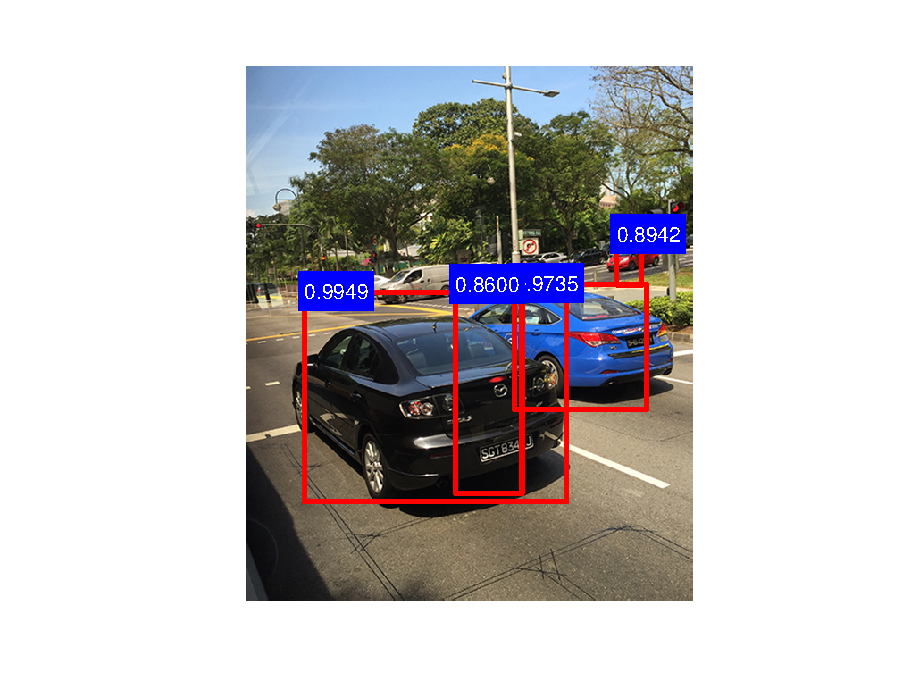
\includegraphics[width=4in, fbox]{Chapter1/boundingbox.eps}
\caption{Bounding-box example of cars.}
\label{fig:boundingboxexample} 
\end{figure}


\section{Two}

Advanced-driver-assistance system (ADAS) plays an important role in newly designed smart cars to reduce road fatalities by minimizing human error. ADAS systems use in-vehicle cameras to capture the real-time images of roads~\cite{ziebinski2016survey}. Captured images will be handled by detection module, which recognizes lane outlines and road markings, and then respond to drivers accordingly. Current detection algorithms in deep learning are led by CNN-like network, e.g. RCNN~\cite{girshick2014rich} and its variance f-RCNN~\cite{girshick2015fast}. We also start from this structure.

There are several common issues in aforementioned detection process. 

First is extreme weather and bad illumination conditions. In raining days, images captured by ADAS’s camera may be blurry or be stained by raindrops, and the water on the road may lead to reflection of lights. In dusk, sun is dim, and the scene is dark-some. The road markings and lane outlines cannot be distinguished from background easily. With such distortions, the detection algorithm cannot see roads accurately. Consequently, taking measures to denoising is of vital importance. 

Second is curved road. Traditional lane detection algorithms usually work well on straight lane but will meet performance drop once the road turns quickly. VPGNet~\cite{lee2017vpgnet} used vanishing point information to solve this problem. Vanishing point is the visual intersection of two parallel lines~\cite{barnard1983interpreting}, here it is treated as the unseen end of the road.  Inspired by the intuition that human eyes utilize the vanishing point to predict the road trending, VPGNet tried to feed this information into neural network by multi-task method. They use multi-task because features employed by VP task, like road curving angle and trending, may also be useful in the detection of lanes and road markings. Based on this, we can expect that with VP information given, the Neural Network can converge better on the other two tasks (lane detection, road marking detection). But VPGNet’s VP feeding scheme is simple, not as efficient as expected. We proposed a new scheme to train with VP information.

\section{Related Work}


\subsection{Benchmarks}

Some well-labeled datasets for lanes and road marking were collected in work \cite{caltech, lee2017vpgnet}

First, the caltech lane detection dataset \cite{caltech} has 1,225 photos captured in two cities, washington and cordova. It features various types of lanes (straight, curved, paralleled). But this dataset has no label for traffic symbols, and no much photo under extreme weather conditions. Later on, VPGNet \cite{lee2017vpgnet} made improvements on benchmark building. They collected 20,386 images under various weather and illumination conditions. Besides, VPGNet has more information on road markings and vanishing points. It uses 1 channel to label 18 classes of lanes and road markings, and 1 channel for vanishing point information.

\subsection{Classical Lane Detection}

There are several ways to get the information for lane detection and prediction usage, such as Monocular vision, stereo, LIDAR, inertial measurement unit (IMU) combined with information obtained from global positioning system (GPS) and high resolution digital maps. \cite{hillel2014recent}. In our work we focus on Monocular vision (Single camera).

In previous work, researchers found relation between wheeling and gaze direction when driving. Human employs the distant region to estimate the road curvature \cite{land1995parts}. Also, the gaze direction relies on the 'tangent point' on the inside of each curve when driving on curvature of the road ahead \cite{land1994we}. This gives possible to utilize the unseen vanishing point in lane prediction.

\subsection{Deep-learning based Object Detection}

Lane and road marking detection tasks are within the scope of object detection, so algorithms popular in object detection have been implemented in lane detection \cite{tang2020review}. 

Recent years, with the DCNN like AlexNet \cite{krizhevsky2012imagenet} being brought up, deep learning has been driving significant progress in the object detection area. Later RCNN and its variants \cite{girshick2014rich, girshick2015fast, ren2015faster} integrates CNN with the region proposal selective search; GoogLeNet \cite{szegedy2015going} and VGGNet \cite{simonyan2014very} gained improvement with deeper encoder. With the network going deeper, computational efficiency becomes the main problem. More powerful network architectures such as ResNets \cite{he2016deep}, DenseNets \cite{huang2017densely} and Inception \cite{ioffe2015batch} have been proposed, which combine path blocks to reduce the number of parameters while improving the accuracy. Most recently, DETR \cite{carion2020end} combined the CNN with transformer architecture, taking the object detection problem as a set-set mapping and achieved promising results on big-object detection.

Lanes are thin and small objects, thus general methods sometimes work bad \cite{tang2020review}. There are some researches featured in picking out small items. U-Net \cite{ronneberger2015unet} extracts the feature map from encoding path and attach it with the decoding path, by which method the network can keep context for local features.

Efforts to use the neural network in lane detection tasks have also been proved solid. Work \cite{borji2016vanishing} first used the CNN structure to predict the vanishing point, and VPGNet \cite{lee2017vpgnet} employed vanishing point information by multi-task method to enhance the prediction of the lanes.

\section{Four}

\subsection{Six}


%=== END OF CHAPTER SIX ===
\end{spacing}
\newpage
